
\chapter{Functions and Datasets}

\section{Analytical Functions}
\label{sec:functions}

Analytical functions---see~\cref{tab:functions}---with increasing numbers of input dimensions are presented, namely: \textit{(i)} \textit{Rosenbrock} ; \textit{(ii)} \textit{Michalewicz} ; \textit{(iii)} \textit{Branin} ; \textit{(iv)} \textit{Ishigami} ; and \textit{(v)} \textit{g-function}~\cite{molga2005,ishigami1990,Saltelli2007,legratiet2016,forrester2008a}. They are all widely used because they are nonlinear and nonmonotonic. Moreover, two versions of the \emph{g-function} 11-D are also used. \textit{g-function (i)} 11-D demonstrates the behaviour of the methods with a small number of input parameters contributing to the QoI, whereas \textit{g-function (ii)} 11-D exhibits more influent input parameters.

\begin{table}[ht]
\centering
\setcellgapes{5pt}
\makegapedcells
\begin{tabular}{lll}
\toprule
Function&Hypercube & Definition \\
\cmidrule{1-3}
\textit{Rosenbrock} 2-D& $[-2.048, 2.048]^2$ & $
f(X_1, X_2) = \sum_{i = 1}^{d-1}[100(x_{i+1} - x_i^2)^2  +(x_i -1)^2]$\\
\textit{Michalewicz} 2-D& $[0, \pi]^2$ & $
f(X_1, X_2) = -\sum_{i=1}^d \sin(x_i)\sin^{2m}\left(\frac{ix_i^2}{\pi}\right)$\\
\textit{Branin} 2-D& $[-5, 10] \times [0, 15]$ &
$\begin{multlined}[t][0.6\linewidth]
f(X_1, X_2) = \left( x_2 - \frac{5.1}{4\pi^2}x_1^2 + \frac{5}{\pi}x_1 - 6
              \right)^2\\[-1ex]
+ 10 \left[ \left( 1 - \frac{1}{8\pi} \right) \cos(x_1) + 1 \right] + 5x_1\hfill
\end{multlined}$\\
\textit{Ishigami} 3-D& $[-\pi, \pi]^3$ & $ f(X_1, X_2, X_3) = \sin X_1 + 7 \sin^2 X_2 + 0.1 X_3^4 \sin X_1 $\\
\textit{g-function} 4-D& $[0, 1]^4$ & $
f(X_1, X_2, X_3, X_4) = \prod_{i=1}^4 \frac{\lvert 4X_i - 2\rvert + a_i}{1 + a_i}, \quad a_{i} = i$\\
\textit{g-function (i)} 11-D & $[0, 1]^{11}$ & 
$\begin{multlined}[t][0.6\linewidth]
f(X_1, ..., X_{11}) = \prod_{i=1}^{11} \frac{\lvert 4X_i - 2\rvert + a_i}{1 + a_i},\\[-1ex]
\hspace{50pt} \mathbf{a} = [1, 2, 5, 10, 20, 50, 100, 500, 1000, 1000, 1000]\hfill
\end{multlined}$\\
\textit{g-function (ii)} 11-D & $[0, 1]^{11}$ &
$\begin{multlined}[t][0.6\linewidth]
f(X_1, ..., X_{11}) = \prod_{i=1}^{11} \frac{\lvert 4X_i - 2\rvert + a_i}{1 + a_i},\\[-1ex]
\hspace{51pt} \mathbf{a} = [1, 2, 2, 3, 3, 10, 50, 50, 50, 100, 100]\hfill
\end{multlined}$\\
\bottomrule
\end{tabular}
\caption{Analytical functions considered sorted by increasing number of input parameters.}
\label{tab:functions}
\end{table}

\section{Datasets}
\label{sec:dataset}

\Cref{tab:dataset} presents two datasets. The first dataset (El Ni\~no) has no input-output relation and only features a temporal output. The second dataset Hydrodynamics features an input-output relation with spatially varying output. The datasets are as follows:
\begin{itemize}
\item The \emph{El Ni\~{n}o} dataset is a well-known functional dataset~\citep{Hyndman2009}. It consists in a time series of monthly averaged Sea Surface Temperature (SST) in degrees Celsius spatially averaged over the Pacific Ocean region (0-10°S and 90-80°W) from January 1950 to December 2007. The response variable is a vector of size 12 and the data set gathers 58 realizations. Data originate from NOAA ERSSTv5's database available at \href{http://www.cpc.ncep.noaa.gov/data/indices}{http://www.cpc.ncep.noaa.gov/data/indices}.
\item The \emph{Hydrodynamics} dataset gathers water levels (in m) computed with the 1-dimensional Shallow Water Equation MASCARET solver (opentelemac.org) for a 50~km reach of the Garonne river in South-West of France~\citep{Roy2017c}. Uncertain inputs relate to 4 scalars: the friction coefficients of the river bed $Ks1, Ks2, Ks3$ defined over three homogeneous spatial areas, and the upstream boundary condition described by a constant scalar value for the inflow $Q$ in stationary flow. The response variable is a vector of size 463 (number of computation nodes for the 1D mesh) and an ensemble of 200 realizations is considered here. 
\end{itemize}

\begin{table}[!ht]
\centering
\begin{tabular}{lccc}
\toprule
Dataset & Scalar input & Functional output & Sample size\\
\midrule % \cmidrule{2-3}
El Ni\~no & - & 12 & 58\\
Hydrodynamics & 4 & 463 & 200\\
\bottomrule
\end{tabular}
\caption{Description of the El Ni\~no and Hydrodynamics datasets.}
\label{tab:dataset}
\end{table}

\chapter{Optimization Method}
\label{sec:optim_method}

Among the numerous methods that can be used to do an optimization~\cite{Cavazzuti2013} are the one taking advantages of a surrogate model~\cite{forrester2009}. When dealing with complex cases, the numerical cost is such that only a limited number of simulations can be performed. However, ensuring the convergence of an optimization requires a minimal number of such evaluations for both deterministic and stochastic methods. In this context, building a proxy of the simulation setup allows overcoming the computational cost. As this proxy is being used for optimizing the problem, its quality is paramount. At some point refining the space of parameters---leading to a quality improvement of the model---can improve the optimization.

Batman~\cref{chap:batman} was used to handle all the workflow from the design of experiments, to the creation of the surrogate and the optimization. Its workflow is presented in~\cref{alg:workflow}.

\begin{algorithm}
  \caption{Workflow using BATMAN}
  \label{alg:workflow}
  \begin{algorithmic}[1]
  \Require $N_{max}$, $N_s$
  \State Formulate the surrogate $\mathcal{M}$ on $N_s$' output
  \While{$N_s < N_{max}$}
    \State $\mathbf{x_{*}}$ $\gets$ optimization
    \State Compute a new sample at $\mathbf{x_{*}}$
    \State Update the surrogate $\mathcal{M}$
  \EndWhile
  \end{algorithmic}
\end{algorithm}

\emph{Efficient Global Optimization} (EGO)~\cite{jones1998} is a Bayesian optimization taking into account the variance of the model. The objective of the optimization is to improve the current solution $Y_{\min}$. The improvement is computed as:
\begin{align}
I(\mathbf{x}) \left\{\begin{array}{rcl} Y_{\min} - \hat{Y}(\mathbf{x}) & \text{if } \hat{Y}(\mathbf{x}) < Y_{\min} \\ 0   & \text{otherwise} \end{array}\right. .
\end{align}

Using the surrogate, the prediction is expressed as a random process with $Y\sim \mathbb{N}(\hat{Y}, s^2)$. Thus, the objective is to get the maximal mean improvement. The expected improvement (EI) is computed as a tradeoff between the minimal value $Y_{\min}$ and an expected value given by the standard error $s$ for a given prediction $\hat{Y}$. It reads:
\begin{align}
\mathbb{E}[I(\mathbf{x})] = (Y_{\min} - \hat{Y})\Phi \left( \frac{Y_{\min} - \hat{y}(\mathbf{x})}{s} \right) + s\phi \left( \frac{Y_{\min} - \hat{Y}(\mathbf{x})}{s} \right), 
\end{align}
\noindent with $\phi(.), \Phi(.)$, respectively, the Probability Density Function (PDF) and Cumulative Distribution Function (CDF) of the normal distribution. Selecting the point with the highest expected improvement is achieved either: \emph{(i)} by maximizing the difference between the minimal value and the predicted response; or \emph{(ii)} by increasing the standard deviation---see~\cref{fig:branin_ego}. Hence, the first component is said to \emph{exploit} the model while the other seeks to \emph{explore} it. These two phases are here automatically selected. In~\cite{schonlau1998}, they proposed with the \emph{Generalized Expected Improvement} a way to define a constant $g$ to adjust the degree of \emph{exploration vs exploitation}: $\mathbb{E}[I^g]$. The highest $g$ is, the more exploratory the strategy is. Indeed, the initial EI strategy tends to add too much effort at improving the current solution and only then consider other regions of the parameters space. But this raises another concern about the value of this constant.

\begin{figure}[!ht]               
\centering
\subfloat[Response surface of the Branin function]{
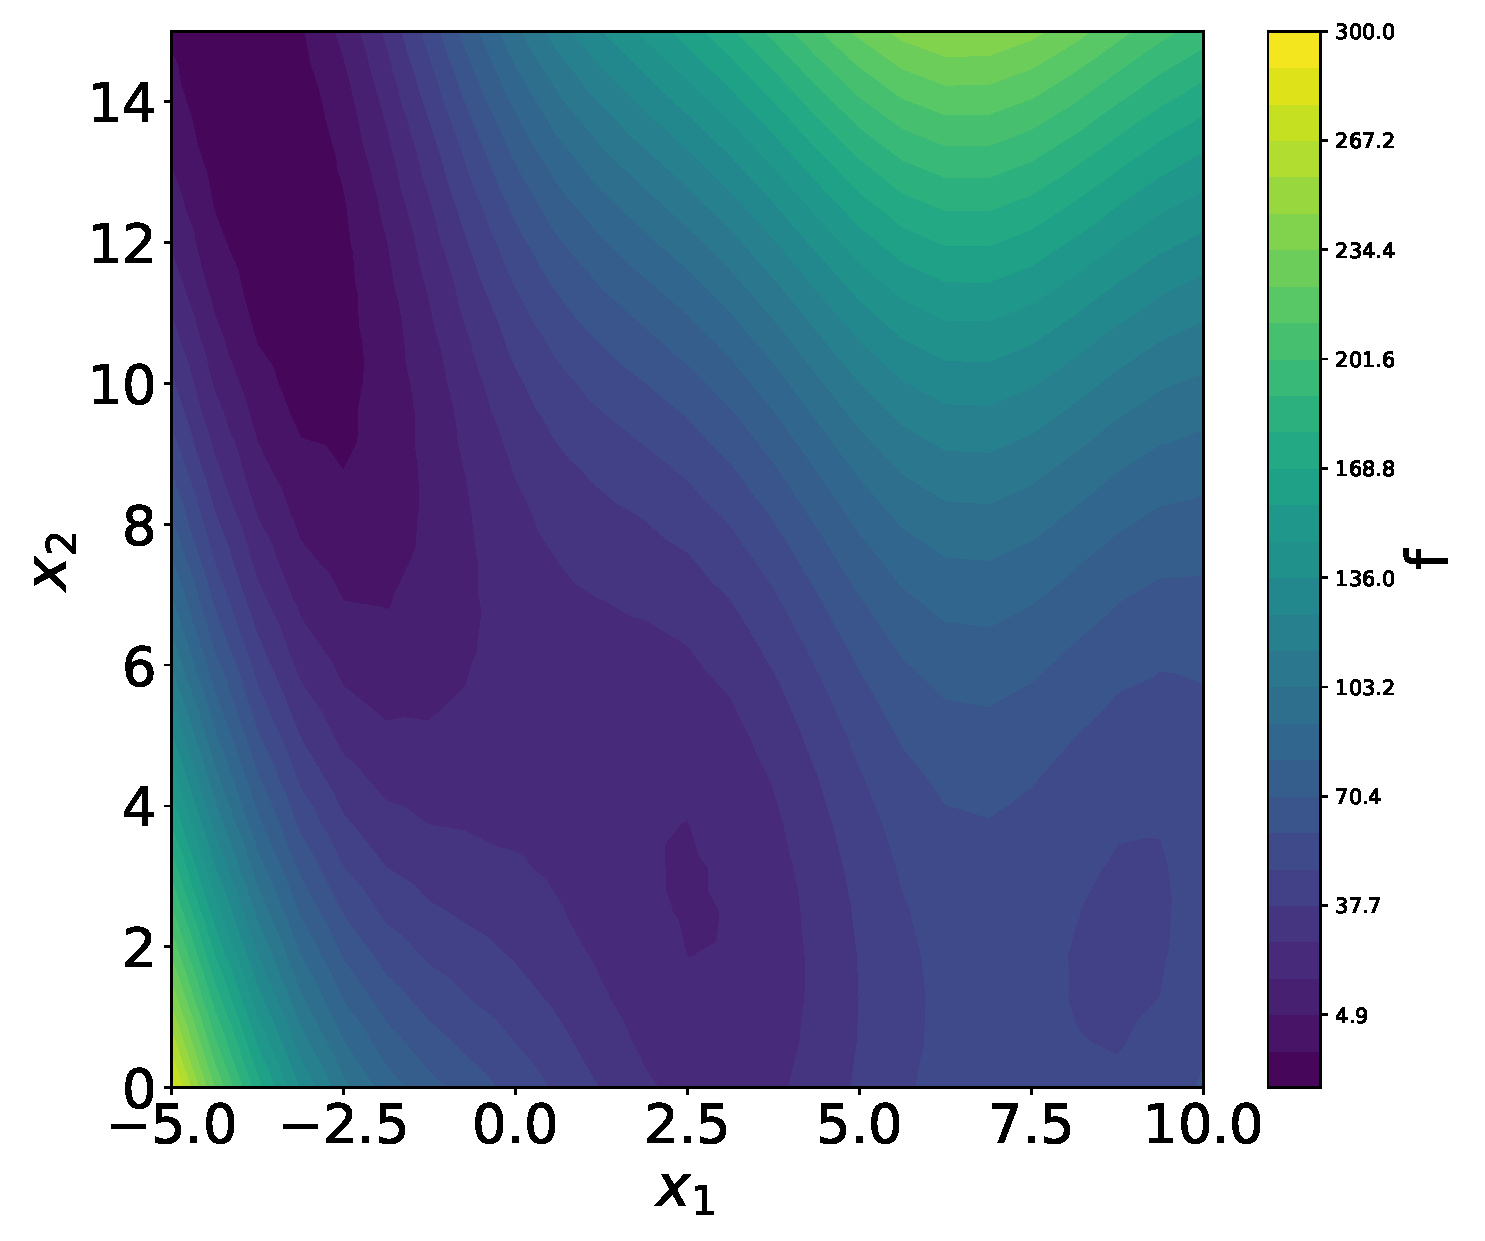
\includegraphics[width=0.6\linewidth,height=\textheight,keepaspectratio]{fig/applications/optim/branin_forrester.pdf}}
   
\subfloat[EGO]{
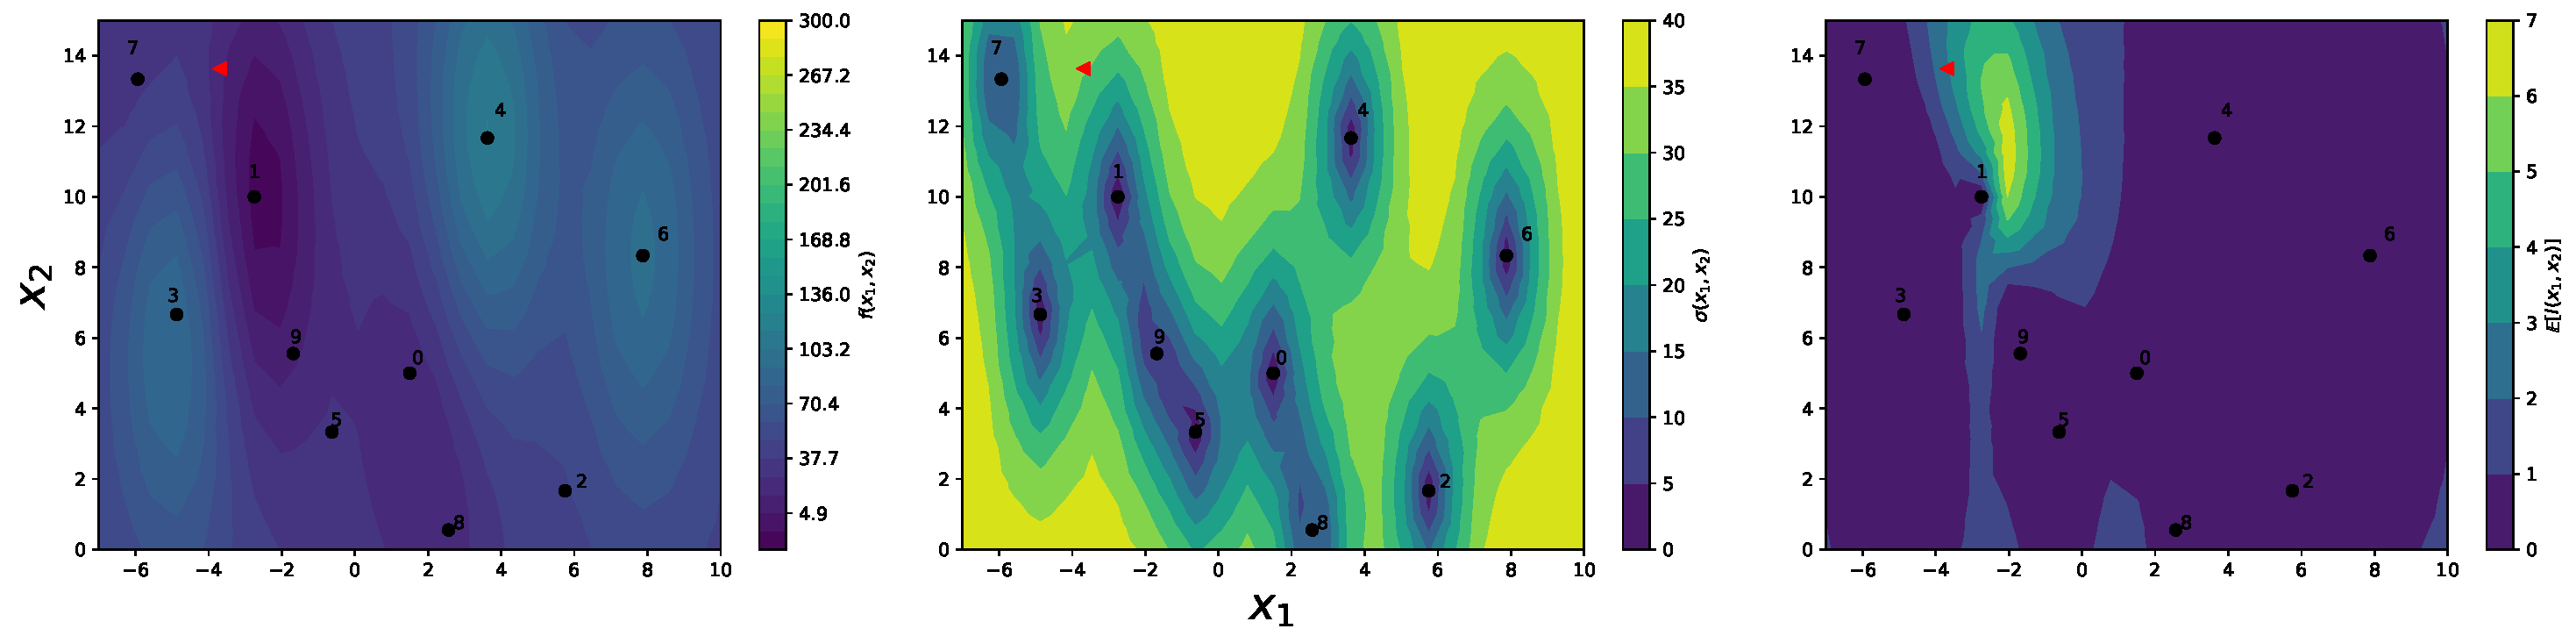
\includegraphics[width=\linewidth,height=\textheight,keepaspectratio]{fig/applications/optim/branin_forrester_ego.pdf}}
\caption{Visualization of EGO on the Branin function---see~\cref{sec:functions}. \emph{Left} is the response surface of the current surrogate model constructed using samples represented by \emph{black dots}. \emph{Center} is the variance of the GP surrogate. \emph{Right} is the expected improvement. The \emph{red triangle} represents the global optimum of the function.}
\label{fig:branin_ego}
\end{figure}

Thus, in this work we used the classical expected improvement formulation in order to avoid the definition of an additional constant. Due to the computational cost of the simulations, this parameter was not characterized.

